\documentclass{standalone}
\usepackage{tikz}
\usetikzlibrary{shapes, backgrounds}
\begin{document}
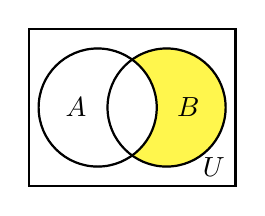
\begin{tikzpicture}
    % Define the universe as a rectangle
    \draw[thick, fill=white] (0,0) rectangle (2.625,2);
    % Draw A
    \draw[fill=white] (0.875,1) circle (0.75);
    % Draw B
    \draw[fill=white] (1.75,1) circle (0.75);
    % A complement intersect B area
    \begin{scope}
        \clip (0,0) rectangle (2.625,2);
        \fill[yellow!70] (1.75,1) circle (0.75);
        \begin{scope}
            \clip (0.875,1) circle (0.75);
            \fill[white] (1.75,1) circle (0.75);
        \end{scope}
    \end{scope}

    % Labels
    \node[align=center] at (0.6,1) {$A$};
    \node[align=center] at (2.025,1) {$B$};
    \node[align=center] at (2.35,0.25) {$U$};

    % Draw borders
    \draw[draw=black, thick] (0.875,1) circle (0.75);
    \draw[draw=black, thick] (1.75,1) circle (0.75);
\end{tikzpicture}
\end{document}